\documentclass[tikz,border=2mm]{standalone}
\begin{document}
	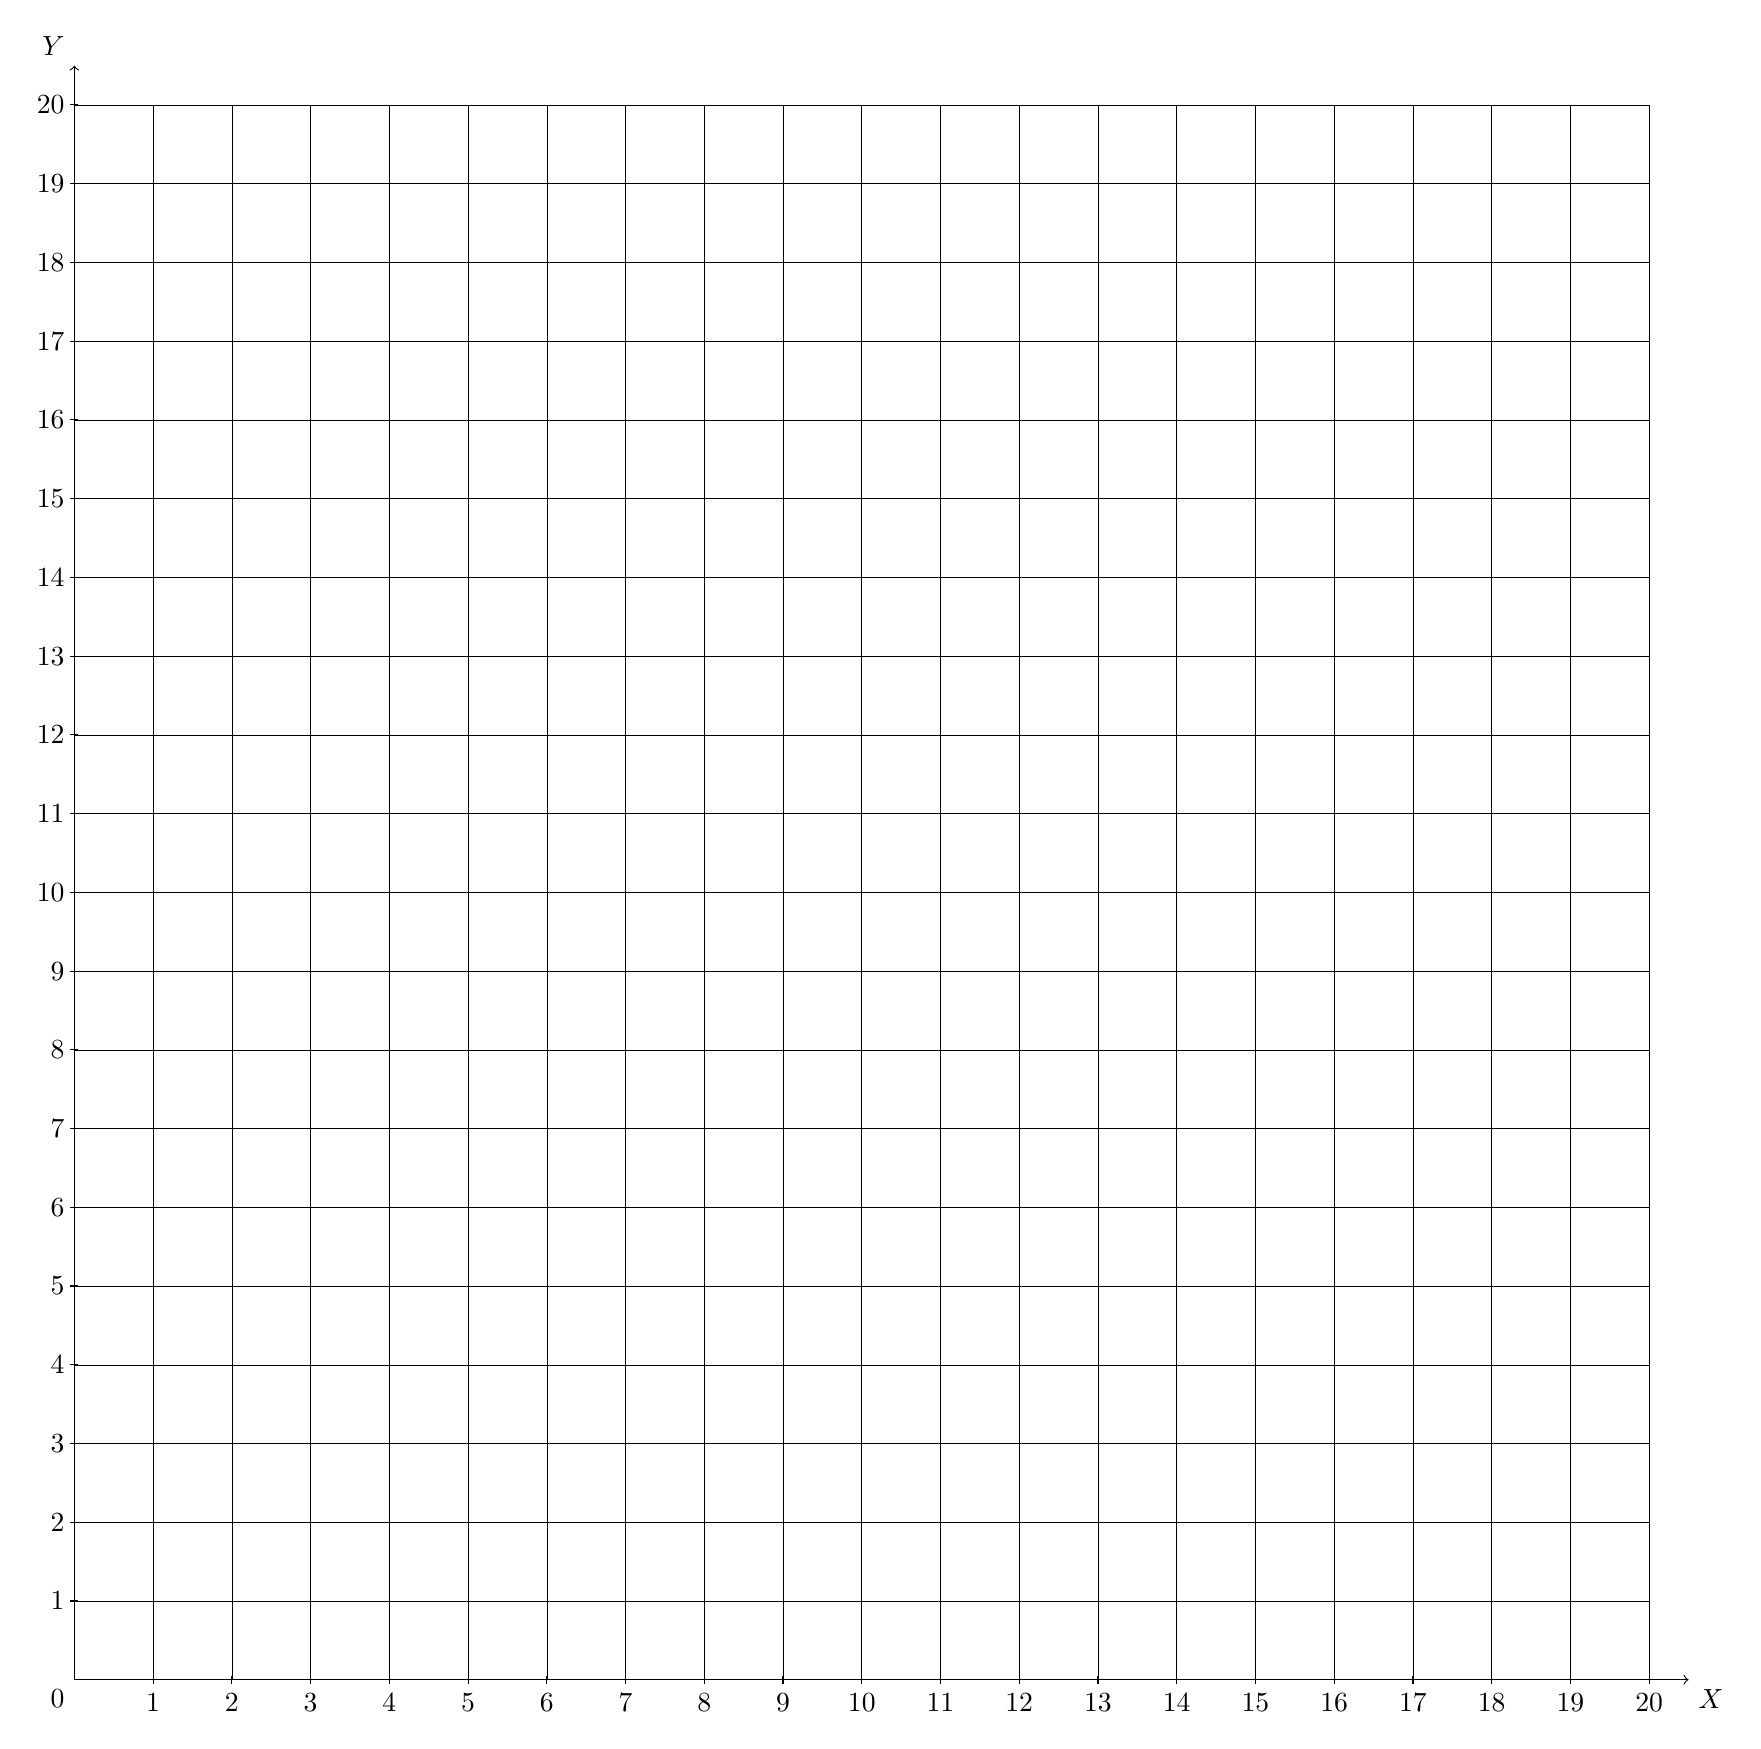
\begin{tikzpicture}
		\draw[help lines,black] (0,0) grid (20,20); %网格线
		\draw [->] (0,0)--(20.5,0) node[below right] { $X$};
		\draw [->] (0,0)--(0,20.5) node[above left] {$Y$};
		\node[below left] at (0,0) {0};
		\foreach \i in {1,...,20}
		\draw (\i,-0.05)--++(90:0.1) node[below=1mm]{\i};
		\foreach \i in {1,...,20}
		\draw (0.05,\i)--++(180:0.1) node[left=-0.5mm]{\i};
	\end{tikzpicture}    
\end{document}
